\chapter{Einführung}
\label{cha:Einfuehrung}

Der technologische Prozess einer Kältemaschine ermöglicht es einer Wärmequelle Wärme  auf einem niedrigen Temperaturniveau zu entziehen und diese an eine Wärmesenke auf einem höheren Temperaturniveau wieder abzugeben. Um diesen thermodynamischen Prozess zu ermöglichen, muss dem  Kältekreislauf, nach dem 2. Hauptsatz der Thermodynamik, Energie hinzugefügt werden. 

Im Jahre 2009 waren alleine in Deutschland 129 Millionen Kältemaschinen in Gebrauch. 70 Prozent dieser Kältemaschinen wurden elektrisch angetrieben. Die wichtigste Technologie zur Erzeugung von Kälte die Kompressionskälteanlage. Der Energieverbrauch für den Betrieb aller Kältemaschinen wird von Preuss \citep{Preuss2011} für das Jahr 2009  auf  ca. 72 Mrd. kWh geschätzt. Dies entspricht ca. 15 $\%$ des nationalen Stromverbrauchs.  Abbildung \ref{fig:Aufteilung nach Einsatzgebiet} zeigt die Aufteilung der sich in Betrieb befindenden Kältemaschinen auf ihre Einsatzgebiete mit anteiligem Energieverbrauch für das Jahr 2009 in Deutschland. \citep{EnergieAgenturNRW2010}

\begin{figure}[htb]
	\centering
		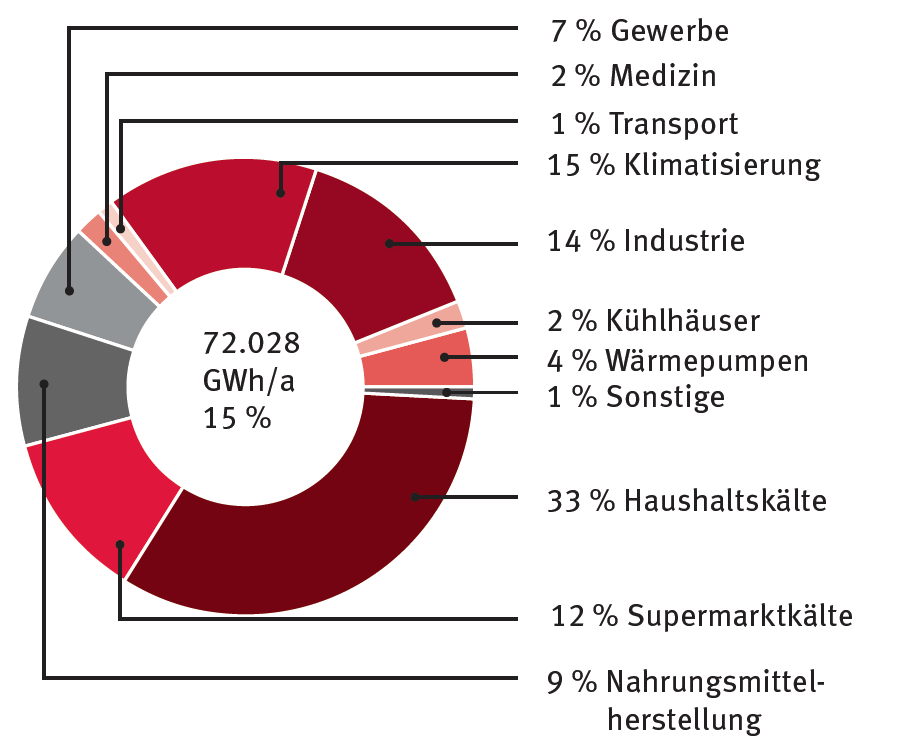
\includegraphics[width=0.570\textwidth]{Pictures/Energieverbrauch_Aufteilung_Karlsruhe.png}
	\caption{Aufteilung der sich in Deutschland in Betrieb befindenden Kältemaschinen je nach Einsatzgebiet und Energieverbrauch im Jahre 2009. \citep{M.Stoeckner2012} \citep{Preuss2011}}
	\label{fig:Aufteilung nach Einsatzgebiet}
\end{figure}

Der Kälteleistungsbedarf ist nach wie vor ansteigend, womit eine größere Klimabelastung einhergeht. Auf der einen Seite entsteht eine steigende CO$_{2}$-Belastung für die Bereitstellung der Antriebsenergie der Kältemaschinen. Auf der anderen Seite stellt die Belastung der Umwelt durch ungewollte direkte Kältemittelemissionen mit teils hohen CO$_2$-Äquivalenten eine Herausforderung dar.

Im Bezug auf Kältemaschinen werden in der Literatur eine Vielzahl an Möglichkeiten und Potentialabschätzungen zur Senkung des Energieverbrauches und der Umweltbelastung genannt. Von der Verwendung von natürlichem Kältemittel, Wärmerückgewinnung vom Verflüssiger sowie von Downsizing des Kompressors ist die Rede. Laut EnergieAgentur.NRW \citep{EnergieAgenturNRW2010} entfallen bei der elektrischen Leistungsaufnahme einer Kälteanlage im Kühlbetrieb durchschnittlich:

\begin{itemize}
	\item ca. 88 $\%$ auf den Kompressor,
	\item ca. 7 $\%$ auf den Verflüssiger,
	\item ca. 5 $\%$ auf den Verdampfer.
\end{itemize}

Die Energieverbrauch des Verflüssigers bzw. Verdampfers wird durch deren eingebauten Ventilator bestimmt. 
Folglich ist der Kompressor der größte Energieverbaucher in einer Kälteanlage. Um eine effiziente Kälteanlage zu betreiben, sollte die zu verrichtende Arbeit vom Kompressor so niedrig wie möglich gehalten werden.

Ziel dieser Arbeit ist der Aufbau, die Inbetriebnahme und erste Test für ein Messsystem, das sowohl Vereisungs- als auch Abtauversuche für verschiedene Luftkühler durchführen kann. Vereiste Luftkühler führen zu einem Leistungsabfall der Kälteleistung. \cite{Grote2014}Dadurch muss der Luftkühler zu bestimmten Zeiten abgetaut werden, um das Eis von dem Wärmeübertrager zu entfernen und die ursprüngliche Kälteleistung wieder zur Verfügung stellen zu können. 



